\let\negmedspace\undefined
\let\negthickspace\undefined
\documentclass[journal,12pt,twocolumn]{IEEEtran}
\usepackage{cite}
\usepackage{amsmath,amssymb,amsfonts,amsthm}
\usepackage{algorithmic}
\usepackage{graphicx}
\usepackage{textcomp}
\usepackage{xcolor}
\usepackage{txfonts}
\usepackage{listings}
\usepackage{enumitem}
\usepackage{mathtools}
\usepackage{gensymb}
\usepackage[breaklinks=true]{hyperref}
\usepackage{tkz-euclide} % loads  TikZ and tkz-base
\usepackage{listings}



\newtheorem{theorem}{Theorem}[section]
\newtheorem{problem}{Problem}
\newtheorem{proposition}{Proposition}[section]
\newtheorem{lemma}{Lemma}[section]
\newtheorem{corollary}[theorem]{Corollary}
\newtheorem{example}{Example}[section]
\newtheorem{definition}[problem]{Definition}
%\newtheorem{thm}{Theorem}[section] 
%\newtheorem{defn}[thm]{Definition}
%\newtheorem{algorithm}{Algorithm}[section]
%\newtheorem{cor}{Corollary}
\newcommand{\BEQA}{\begin{eqnarray}}
\newcommand{\EEQA}{\end{eqnarray}}
\newcommand{\define}{\stackrel{\triangle}{=}}
\theoremstyle{remark}
\newtheorem{rem}{Remark}
%\bibliographystyle{ieeetr}
\begin{document}
%
\providecommand{\pr}[1]{\ensuremath{\Pr\left(#1\right)}}
\providecommand{\prt}[2]{\ensuremath{p_{#1}^{\left(#2\right)} }}        % own macro for this question
\providecommand{\qfunc}[1]{\ensuremath{Q\left(#1\right)}}
\providecommand{\sbrak}[1]{\ensuremath{{}\left[#1\right]}}
\providecommand{\lsbrak}[1]{\ensuremath{{}\left[#1\right.}}
\providecommand{\rsbrak}[1]{\ensuremath{{}\left.#1\right]}}
\providecommand{\brak}[1]{\ensuremath{\left(#1\right)}}
\providecommand{\lbrak}[1]{\ensuremath{\left(#1\right.}}
\providecommand{\rbrak}[1]{\ensuremath{\left.#1\right)}}
\providecommand{\cbrak}[1]{\ensuremath{\left\{#1\right\}}}
\providecommand{\lcbrak}[1]{\ensuremath{\left\{#1\right.}}
\providecommand{\rcbrak}[1]{\ensuremath{\left.#1\right\}}}
\newcommand{\sgn}{\mathop{\mathrm{sgn}}}
\providecommand{\abs}[1]{\left\vert#1\right\vert}
\providecommand{\res}[1]{\Res\displaylimits_{#1}} 
\providecommand{\norm}[1]{\left\lVert#1\right\rVert}
%\providecommand{\norm}[1]{\lVert#1\rVert}
\providecommand{\mtx}[1]{\mathbf{#1}}
\providecommand{\mean}[1]{E\left[ #1 \right]}
\providecommand{\cond}[2]{#1\middle|#2}
\providecommand{\fourier}{\overset{\mathcal{F}}{ \rightleftharpoons}}
\newenvironment{amatrix}[1]{%
  \left(\begin{array}{@{}*{#1}{c}|c@{}}
}{%
  \end{array}\right)
}
%\providecommand{\hilbert}{\overset{\mathcal{H}}{ \rightleftharpoons}}
%\providecommand{\system}{\overset{\mathcal{H}}{ \longleftrightarrow}}
	%\newcommand{\solution}[2]{\textbf{Solution:}{#1}}
\newcommand{\solution}{\noindent \textbf{Solution: }}
\newcommand{\cosec}{\,\text{cosec}\,}
\providecommand{\dec}[2]{\ensuremath{\overset{#1}{\underset{#2}{\gtrless}}}}
\newcommand{\myvec}[1]{\ensuremath{\begin{pmatrix}#1\end{pmatrix}}}
\newcommand{\mydet}[1]{\ensuremath{\begin{vmatrix}#1\end{vmatrix}}}
\newcommand{\myaugvec}[2]{\ensuremath{\begin{amatrix}{#1}#2\end{amatrix}}}
\providecommand{\rank}{\text{rank}}
\providecommand{\pr}[1]{\ensuremath{\Pr\left(#1\right)}}
\providecommand{\qfunc}[1]{\ensuremath{Q\left(#1\right)}}
	\newcommand*{\permcomb}[4][0mu]{{{}^{#3}\mkern#1#2_{#4}}}
\newcommand*{\perm}[1][-3mu]{\permcomb[#1]{P}}
\newcommand*{\comb}[1][-1mu]{\permcomb[#1]{C}}
\providecommand{\qfunc}[1]{\ensuremath{Q\left(#1\right)}}
\providecommand{\gauss}[2]{\mathcal{N}\ensuremath{\left(#1,#2\right)}}
\providecommand{\diff}[2]{\ensuremath{\frac{d{#1}}{d{#2}}}}
\providecommand{\myceil}[1]{\left \lceil #1 \right \rceil }
\newcommand\figref{Fig.~\ref}
\newcommand{\system}[1]{\stackrel{#1}{\xleftrightarrow{\mathcal{L}}}}
\newcommand{\systeminv}[1]{\stackrel{#1}{\xleftrightarrow{\mathcal{L}^{-1}}}}


\newcommand\tabref{Table~\ref}
\newcommand{\sinc}{\,\text{sinc}\,}
\newcommand{\rect}{\,\text{rect}\,}
%%
%	%\newcommand{\solution}[2]{\textbf{Solution:}{#1}}
%\newcommand{\solution}{\noindent \textbf{Solution: }}
%\newcommand{\cosec}{\,\text{cosec}\,}
%\numberwithin{equation}{section}
%\numberwithin{equation}{subsection}
%\numberwithin{problem}{section}
%\numberwithin{definition}{section}
%\makeatletter
%\@addtoreset{figure}{problem}
%\makeatother

%\let\StandardTheFigure\thefigure
\let\vec\mathbf


\bibliographystyle{IEEEtran}
\title{ GATE NM-50 2022}
\author{EE23BTECH11011- Batchu Ishitha$^{*}$% <-this % stops a space
}
\maketitle




\bigskip

\renewcommand{\thefigure}{\theenumi}
\renewcommand{\thetable}{\theenumi}
%\renewcommand{\theequation}{\theenumi}

Q:  Let $y(x)$ be the solution of the differential equation 
\begin{align}
y^{''} - 4y^{'} -12y &= 3e^{5x} 
 \label{eq:ishitha.g22.nm.50.1.eq}
\end{align}
satisfying $y(0)=\frac{18}{7}$ and $y^{'}(0)=\frac{-1}{7}$. \\
Then $y(1)$ is \underline{\hspace{2.5cm}}  (rounded off to nearest integer).      \hfill{GATE NM 2022 }

\solution
\begin{table}[!ht]    
    \centering
    \resizebox{9cm}{1cm}{
        \begin{tabular}[12pt]{ |c| c|c|}
    \hline
    \textbf{Parameter} & \textbf{Description} & \textbf{Value}\\ 
    \hline
    $y^{''} -  4y^{'} -12y = 3e^{5x}$ & Differential equation & none\\
    \hline
    $y\brak{x}$ &Solution of  differential equation & $y(0)=\frac{18}{7}$\\
    \hline
    $y^{'}\brak{x}$ & First order derivative of solution of differential equation & $y^{'}\brak{0}=\frac{-1}{7}$\\
    \hline
     \end{tabular} 
 
    }
    \caption{Input Parameters}
    \label{table:ishitha.g22.nm.50.t1}
\end{table}

\begin{equation}
y^{''}(t) \system{} s^{2}Y(s)-sy(0)-y^{'}(0) \\ \label{eq:ishitha.g22.nm.50.2.eq}
\end{equation}

\begin{equation}
y^{'}(t)  \system{} sY(s)-y(0) \\ \label{eq:ishitha.g22.nm.50.3.eq}
\end{equation}

\begin{equation}
y(t)     \system{}   Y(s) \\ \label{eq:ishitha.g22.nm.50.4.eq}
\end{equation}

\begin{equation}
e^{at}   \system{}  \frac{1}{s-a} \\ \label{eq:ishitha.g22.nm.50.5.eq}
\end{equation}

Applying Laplace transform on both sides of  ~\eqref{eq:ishitha.g22.nm.50.1.eq},
\begin{align}
\mathcal{L}\brak{y^{''}(t) - 4y^{'}(t) -12y(t)}&=\mathcal{L}\brak{3e^{5x}}
\end{align}

From ~\eqref{eq:ishitha.g22.nm.50.2.eq},~\eqref{eq:ishitha.g22.nm.50.3.eq},~\eqref{eq:ishitha.g22.nm.50.4.eq},~\eqref{eq:ishitha.g22.nm.50.5.eq}
\begin{align}
Y(s)\brak{s^{2}-4s-12} -y(0)\brak{s-4} \nonumber \\-y^{'}(0) &= \frac{3}{s-5} \\
Y(s)\brak{s^{2}-4s-12} - \frac{\brak{18s -73 }}{7}  &=\frac{3}{(s-5)} \\
Y(s) = \frac{3}{(s-5)\brak{s^{2}-4s-12}} &+ \frac{\brak{18s -73 }}{7\brak{s^{2}-4s-12} } 
\end{align}

\begin{equation}
\implies Y(s) = \frac{1}{\brak{s-6}} -\frac{3}{7\brak{s-5}} + \frac{1}{\brak{s+2}} \\ \label{eq:ishitha.g22.nm.50.6.eq}
\end{equation}


\begin{equation}
\frac{1}{s-a}   \systeminv{}  e^{at}  \\ \label{eq:ishitha.g22.nm.50.7.eq}
\end{equation}
Now finding Inverse Laplace Transform on both sides of ~\eqref{eq:ishitha.g22.nm.50.6.eq} ,

From ~\eqref{eq:ishitha.g22.nm.50.7.eq}
\begin{align}
\implies y(t) &= \brak{e^{6t} -\frac{3}{7}e^{5t} + 2e^{-2t}}u(t)
\end{align}

\begin{align}
\implies y(1) &= e^{6} -\frac{3}{7}e^{5} + 2e^{-2} \\
\therefore y(1) &= 340
\end{align}

\begin{figure}[!ht]
    \centering
     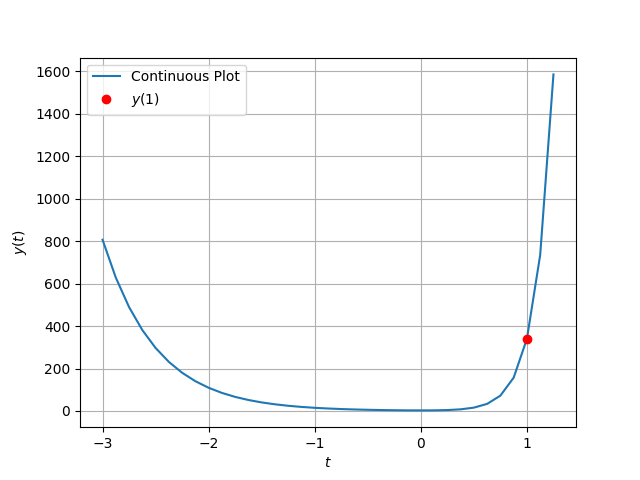
\includegraphics[width=\columnwidth]{./figs/g50fig1.png}
    \caption{}    
    \label{fig:ishitha.g22.nm.50.f2}
\end{figure}
\end{document}
